\documentclass[10pt,a4paper]{article}

\bibliographystyle{ieeetr}

\usepackage[margin=1in]{geometry}
\usepackage{graphicx}
\usepackage{subfig}
\usepackage{amsmath}
\usepackage{url}
\usepackage{pgfgantt}
\usepackage[title]{appendix}
\usepackage{pdfpages}

\graphicspath{{./figs/}}

\newcommand{\code}[1]{\texttt{#1}}

\title{A modular kernel for the Raspberry Pi: Project Specification}
\date{12 October, 2018}

\begin{document}

\maketitle

\begin{center}
    Thomas Archbold \\
    1602581 \\
    University of Warwick \\
\end{center}

\section*{Background}
In most operating systems, many design decisions are made in order to keep
things simple for the user, by keeping most of the technical details hidden. In
most cases, this is an appropriate approach: needlessly offering more choices
for low-level tasks that are usually handled by the operating system, such as
CPU scheduling algorithms, would only serve to confuse the average user. It may
actually be detrimental to the security and the stability of the system by
opening up more opportunities for errors to be introduced.  This more insulated
approach does mean, however, that the user never really knows what is going on
``under the hood'', and indeed whether greater performance can be achieved by
making \textit{different} fundamental decisions.  Furthermore, a number of
operating systems exist for the Raspberry Pi, some focusing on
ease-of-installation, with Linux's NOOBS \cite{NOOBS} distribution, others on
Internet of Things integration, such as the Windows 10 IoT Core distribution
\cite{IoT}. Yet, none exist to serve as an experimental operating system,
designed as a testbed for making and changing these low-level behaviours.  This
project aims to fill this gap for the operating systems enthusiast, one who
wishes to test for themselves the different approaches to CPU scheduling,
interprocess communication, and filesystems. It will give the user the ability
to alter the fundamental ways in which their machine operates by compiling
different modules to handle different tasks, enabling for a more flexible
operating system where such things can be tweaked at any point.

\section*{Main goal}
The goal of this project is to create a modular operating system for the
Raspberry Pi 2 Model B that is capable of loading different modules at
compilation time to tackle CPU scheduling, interprocess communication, and
filesystems in a variety of ways. Specifically, it must have some way to run and
switch between multiple processes using a CPU scheduler; to use both shared
memory and message passing for interprocess communication; to
create, read, update, and delete files and directories using a custom
filesystem; and to interface with the SD card for permanent/mass storage.  To
achieve this, it must implement an interface for compiling different modules,
similar to Linux's \code{insmod}, \code{rmmod}, and Kbuild system \cite{insmod,
Kbuild}.  Furthermore, as executing processes forms a key functional requirement
for the project, there must be a convenient way to load programs into memory and
begin their execution. A solution to this is to implement a basic shell/command
interpreter.

Finally, a key objective of this project will be to get the operating system to
work entirely on real hardware, and not solely in an emulated environment. This
includes booting from the SD card installed in the Raspberry Pi. As the boot
process is handled by the Pi's System on Chip (SoC), booting will be possible
without writing a custom bootloader. On top of booting from it, the operating
system must interact with the SD card in conjunction with a filesystem for
permanent/mass storage. Finally, it must be capable of taking input from a
keyboard connected via USB, and printing output to a physical screen via its
HDMI port.

\subsubsection*{The kernel}
The kernel will be built using the cross-compiler from GCC for
\code{arm-none-eabi}, which provides a toolchain to target the System V
Application Binary Interface (ABI). As a result, programs and fragments of
programs on disk, and by extension the kernel itself, will be in the Executable
and Linkable Format (ELF) after compilation and linking. The kernel will use
just a single core of the four available to the BCM2836, but will support
multithreading, both at the kernel and user levels, with appropriate interfaces
being written in both cases. 

The memory available to the operating system will be organised into pages, and
furthermore it will use a dynamic memory allocator, similar to the C standard
library's \code{malloc()} and \code{free()}, to further split the available
memory into segments. Processes will need to be loaded into and out of memory,
and as such will need an appropriate representation as a Process Control Block
(PCB), and will need to be stored in a Process Table to facilitate context
switching. On top of this, the kernel must also be able to handle interrupts and
exceptions to safely halt processes and bring them out of memory. At this point,
CPU scheduling will need to be tackled, and a long-term and multiple short-term
schedulers implemented. As QEMU does not simulate a system timer, the move to
working on real hardware will coincide with the introduction of multitasking,
involving taking input via USB keyboard and printing output via HDMI.

With the possibility of multiple running processes, synchronisation will need to
be tackled, most likely using semaphores, and the issues of deadlock avoidance,
detection, and correction will need to be considered. Furthermore, solutions for
interprocess communication will then be developed, most likely starting with
shared memory due to its simplicity. Message passing will follow as a
configurable module. Beyond this, a filesystem can then be implemented and
development can move to focus more on user space, including a command
interpreter, actually accessing mass storage, and implementing \code{fork()} and
\code{execute()}. At this time the notion of syscalls and operating system traps
will also need to be developed. As an operating system needs to be written in a
freestanding (as opposed to hosted) environment, a standard library will be
continually developed over the course of the project.

\subsubsection*{Configurable modules}
The project must implement the following as modules, which may be configured at
compilation time by the user:
\begin{itemize}
    \item CPU Scheduling:
        \begin{itemize}
            \item First Come First Served
            \item Round Robin
            \item Shortest Job First
            \item Shortest Remaining Time First
            \item Priority Scheduling (preemptive and non-preemptive)
            \item Lottery Scheduling
        \end{itemize}
    \item Interprocess Communication
        \begin{itemize}
            \item Message passing
            \item Shared memory
        \end{itemize}
    \item Filesystem
        \begin{itemize}
            \item persistent
            \item load-on-request
        \end{itemize}
\end{itemize}

\subsection*{Stretch goals}
Some stretch goals which should be implemented to show understanding of more
complex structures would be some more intricate scheduling algorithms, including
the following \cite{CFS,BFS,DinosaurCPU,Schedulers}:
\begin{itemize}
    \itemsep0em 
    \item Completely Fair Scheduler
    \item Multiple Queue Skiplist Scheduler, MuQSS
    \item Multilevel Queue and Multilevel Feedback Queue
    \item $\mathcal{O}(n)$ Scheduler
    \item $\mathcal{O}(1)$ Scheduler
\end{itemize}

In order to give the operating system more purpose and to increase usability,
the collection of relatively simple programs on offer should be extended,
including a mix of long running CPU- and I/O-bound programs. This will mean that
the relative performance of the schedulers may be seen more easily. While the
Not Recently Used (NRU) algorithm will be used for page replacement due to its
low overhead and decent performance, other algorithms could be explored and
implemented as modules. These may include: First-In-First-Out (to highlight its
poor performance), the Clock Page Replacement algorithm, and the Least Recently
Used algorithm \cite{PageReplacement}.

\subsection*{Further extensions}
Beyond these goals, further extensions would focus on increasing the usability
of the system, and start to shape it into one which someone might actually use
to get things done. One of the simpler ways to achieve this would be to write a
text editor. Additionally, implementing networking into the operating system
would vastly increase its usability and general usefulness. Such goals are
rather far-fetched given the time frame of the project, but would form
meaningful projects later in the life of the operating system.

\subsection*{Out-of-scope}
Features which will not be implemented in the project include graphical user
interfaces and any form of security. Graphics would increase the complexity of
the project too much, and provide too little reward, to be considered a
worthwhile goal. While security would be easier to implement, for example by
following suit of Linux's permissions interface \cite{permissions}, it would
again detract attention from features more in line with the project's goals.
After all, the operating system produced will only be experimental and designed
for use by one user, and as such security will be an unnecessary feature.

\section*{Hardware}
Compared to the Raspberry Pi 1, the Raspberry Pi 2 Model B has:
\begin{itemize}
    \itemsep0em
    \item 900 MHz quad-core ARM Cortex-A7 CPU
    \item 1GB RAM
\end{itemize}
Like the Pi 1 Model B+, it has:
\begin{itemize}
    \itemsep0em
    \item 40 GPIO pins
    \item 4 USB ports
    \item Full HDMI port
    \item MicroSD card slot
    \item 100 Base Ethernet
    \item VideoCore IV graphics Core
    \item Combined 3.5mm audio jack and composite video
    \item Camera interface (CSI)
    \item Display interface (DSI)
\end{itemize}

The main reason for choosing to work with the Raspberry Pi was due to its simple
boot process, details of which can be found here \cite{pi_boot}. In particular,
as it is handled entirely by its SoC, it means a custom bootloader to load the
kernel into memory and transfer control to it will need not be written. The
Raspberry Pi 2 Model B in particular uses the BCM2836 processor, whose
underlying architecture is identical to the 1's BCM2835 and the 3's BCM2837
chips. The only difference is that the 2 uses the quad-core Cortex-A7 cluster as
opposed to the ARM1176JZF-S or the quad-core ARM Cortex-A53 cluster, as used by
the 1 and 3 respectively \cite{BCM2835,BCM2837}.  Therefore, as the choice
between specific models of the Pi would make little significant difference to
the outcome of the project, it made sense to opt for the one already available
to the author at the time the project was conceived, namely the Raspberry Pi 2
Model B.

\begin{figure}[h]
    \begin{center}
        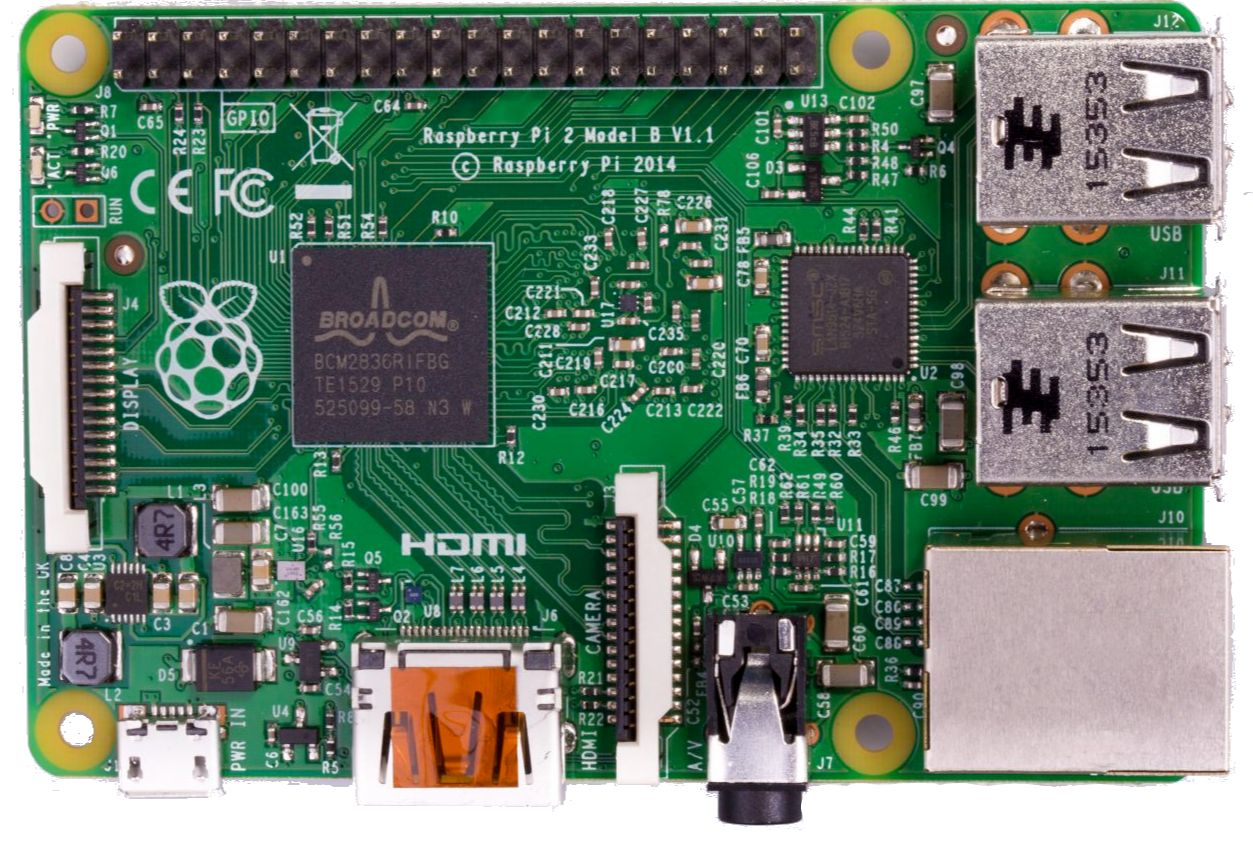
\includegraphics[width=4in]{raspi.png}
        \caption{Raspberry Pi 2 Model B \cite{Pi}}
    \end{center}
\end{figure}

\section*{Methodology}
The methodology best suited to the project will be a mix between plan-driven and
agile approaches. The early stages of the operating system's development will
benefit from the former, as the requirements, such as booting before memory
management before writing scheduling algorithms, will abide by a rigid
structure. An incremental approach will likely be used as opposed to a waterfall
methodology, however, due to its less restrictive nature, and to offer choice
when it is appropriate about what to implement next. After the foundations are
laid, the project will likely move to a more agile approach, where scrum cycles
will be useful both for their flexibility and choice, and their focus on
finishing one aspect of the project at a time.

Throughout the project, regular meetings will be taken with the supervisor to
discuss progress, current problems, and ideas for solutions when necessary.
Organisation will of course be a key aspect to the success of the project, and
the project timetable will be updated to reflect the project's progress. The
meetings will start at once every fortnight in Term 1, and increase to once
weekly in Term 2, simply due to timetabling and course load for other modules.

\section*{Testing}
The project will be tested incrementally. In its early stages, progress will
simply not be able to be made until some systems operate correctly, so thorough
manual testing of such areas will be vital as there will simply not be the
platform to write dedicated unit tests. As it progresses, and unit tests become
more viable, they will be written to cover most likely paths of execution to
identify shortcomings of the system, and dealt with accordingly. Since the
project's aim is to create a configurable operating system, manual testing will
again need to be undertaken in order to verify whether it works under the
various combinations of modules. This will test both the correctness and the
stability of the system rigorously, two of the most important goals of any piece
of software.

\section*{Timetable}
See Appendix.

\ganttset{%
    calendar week text={%
        \pgfcalendarmonthshortname{0}~\startday%
    }%
}

\section*{Technologies}
The following technologies will be used by the project:
\begin{itemize}
    \itemsep0em
    \item Git - version control
    \item Github - to access the project from multiple sources, as well as to
        back it up
    \item C - the language in which most of the operating system will be
        implemented
    \item ARM assembly - used when C is unavailable/inappropriate
        \cite{CannotDoC}
    \item GCC cross compiler for ARM EABI - for cross compiling for the target
        processor, the Cortex-A7 %\cite{CrossCompilation}
    \item QEMU - for emulating the Pi to allow quicker and safer testing
        \footnote{QEMU does not simulate a system timer (at least for the
        Raspberry Pi 2), so some testing will eventually need to be done on real
        hardware}
    \item Make - automate the build process
\end{itemize}

\section*{Resources}
The following documentation will be used throughout for reference to the
architecture of the Cortex-A7 processor and its instruction set, and the
peripherals on the Pi:
\begin{itemize}
    \itemsep0em
    \item Cortex-A7 MPCore Technical Reference Manual
    \item ARM Cortex-A Series Programmer's Guide
    \item Broadcom BCM2835 ARM Peripherals Manual
\end{itemize}

Additional guidance will be taken from the MINIX book \cite{MINIX}, Stanford's
Pintos \cite{Pintos}, and \cite{jsandler}.

\section*{Legal, social, ethical, and professional  considerations}
All software used to build the project is available to use under the GNU Public
License. Throughout the project's development, some testing will be required
from people other than the creator, to gain informal feedback especially with
regards to usability; these people are likely to be friends and colleagues,
hence the social, ethical, and professional issues are insignificant.

\bibliography{bibliography}

\begin{appendices}

\pagenumbering{gobble}  % switch off page numbering

    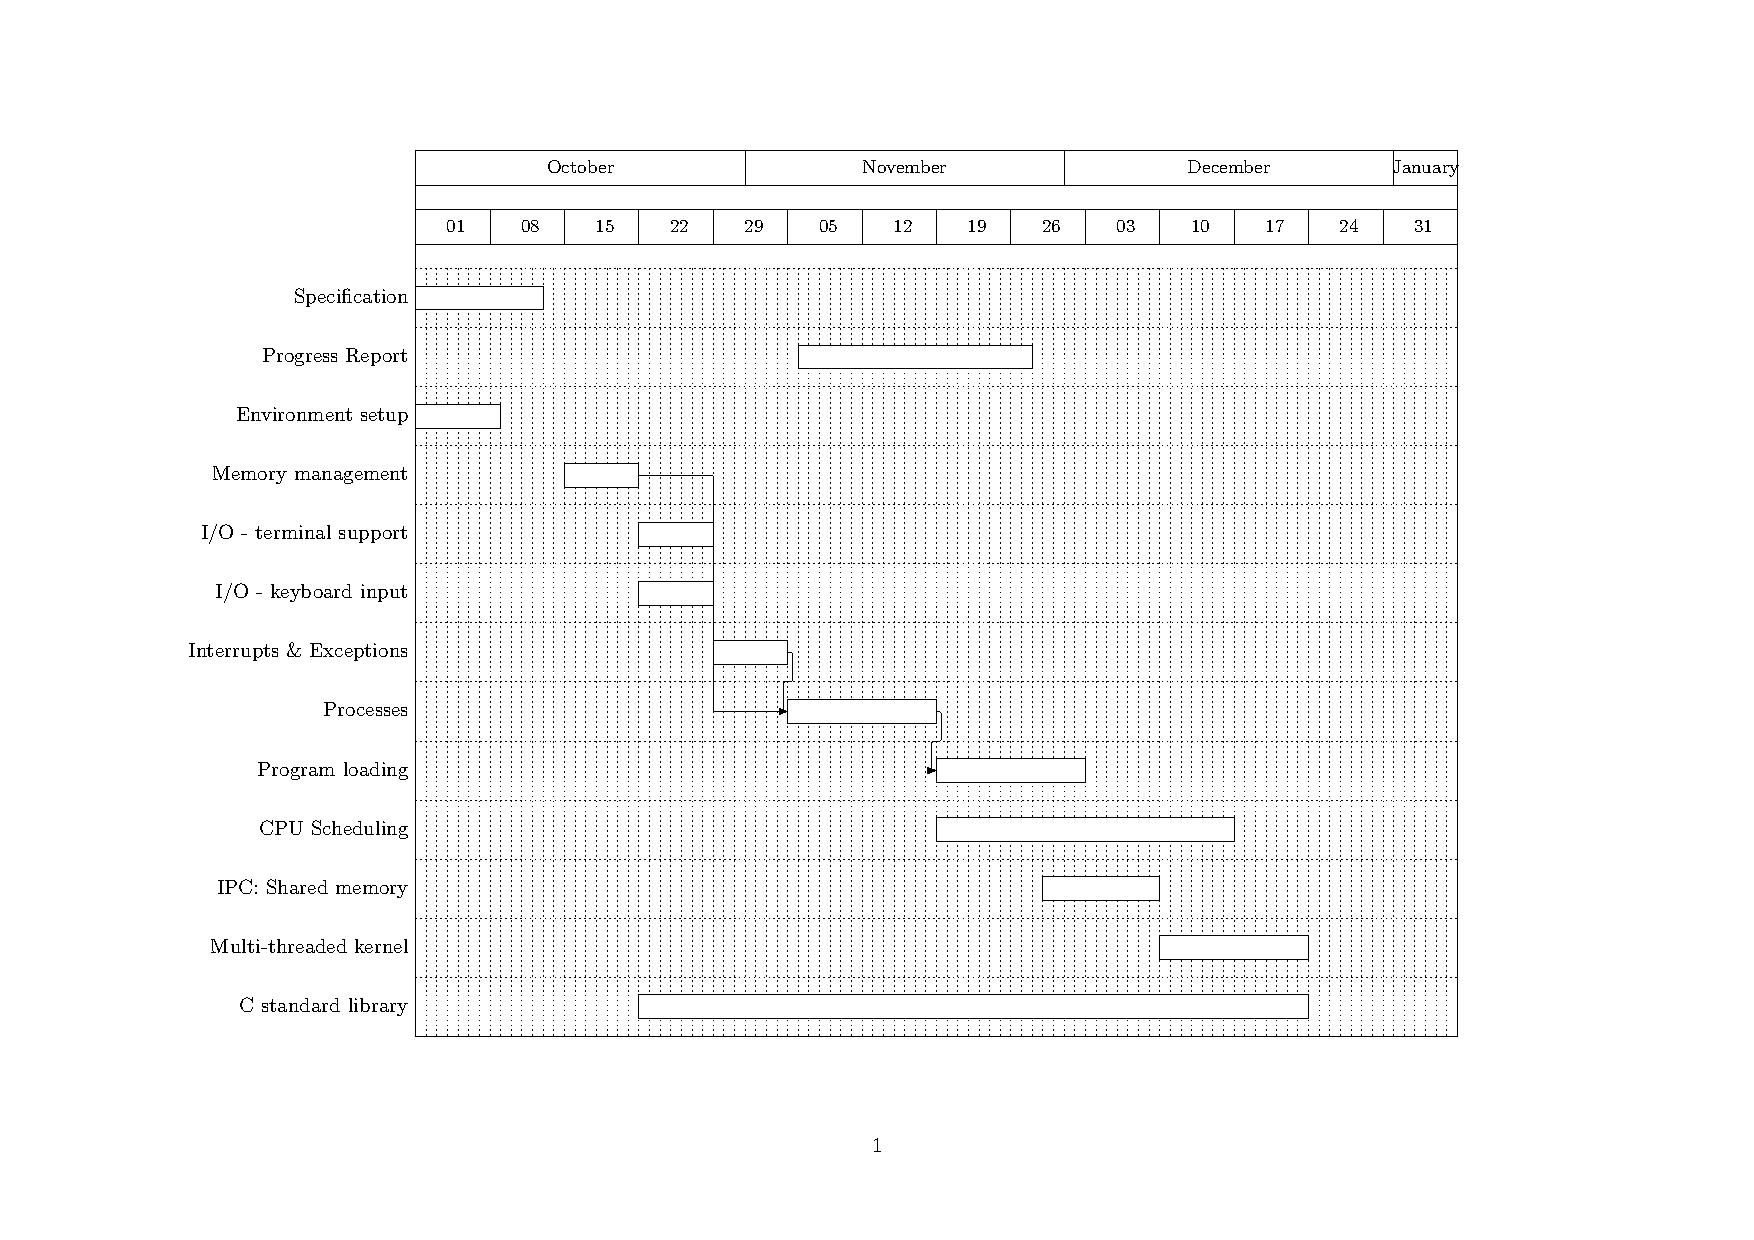
\includepdf[landscape=true,pages=1,pagecommand={\section{Timetable}}]{timetable/timetable.pdf}
    \includepdf[landscape=true,pages=2-,pagecommand={}]{timetable/timetable.pdf}

\end{appendices}

\end{document}
